\documentclass[11pt,letterpaper]{article}
\usepackage[lmargin=1in,rmargin=1in,tmargin=1in,bmargin=1in]{geometry}
\usepackage{../style/homework}
\usepackage{../style/commands}
\setbool{quotetype}{true} % True: Side; False: Under
\setbool{hideans}{false} % Student: True; Instructor: False

\newcommand{\blank}[1]{\underline{\hspace{#1}}} % Blank Underline
\usetikzlibrary{arrows.meta}
\usetikzlibrary{decorations.markings}
% -------------------
% Content
% -------------------
\begin{document}

\homework{18: Due 12/12}{It has been said that geometry is the art of applying good reasoning to bad diagrams.}{Richard J. Trudeau}

% Problem 1
\problem{10} Consider the graph $G$ shown below.
	\[
	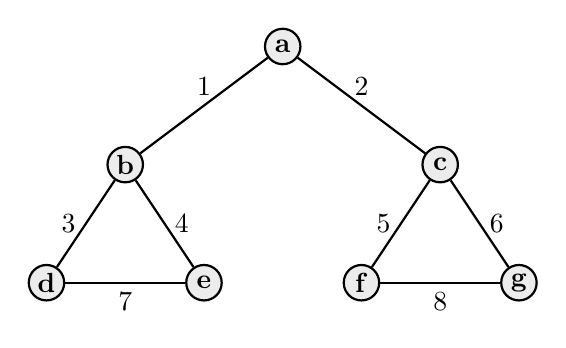
\begin{tikzpicture}
	\begin{scope}[
		every node/.style={circle,thick,fill=gray!15,draw,minimum size = 0.45cm, inner sep=1pt}
	]
	\node (a) at (0,0.5) {$\mathbf{a}$};
	\node (b) at (-2,-1) {$\mathbf{b}$};
	\node (c) at (2,-1) {$\mathbf{c}$};
	\node (d) at (-3,-2.5) {$\mathbf{d}$};
	\node (e) at (-1,-2.5) {$\mathbf{e}$};
	\node (f) at (1,-2.5) {$\mathbf{f}$};
	\node (g) at (3,-2.5) {$\mathbf{g}$};
	\end{scope}
	\begin{scope}[
		>={Stealth[black]},
%		every node/.style={fill=white,circle},
		every edge/.style={draw=black, thick}
	]
	\path [-] (a) edge node[above] {$1$} (b);
	\path [-] (a) edge node[above] {$2$} (c);
	\path [-] (b) edge node[left] {$3$} (d);
	\path [-] (b) edge node[right] {$4$} (e);
	\path [-] (c) edge node[left] {$5$} (f);
	\path [-] (c) edge node[right] {$6$} (g);
	\path [-] (d) edge node[below] {$7$} (e);
	\path [-] (f) edge node[below] {$8$} (g);
	\end{scope}
	\end{tikzpicture}
	\]

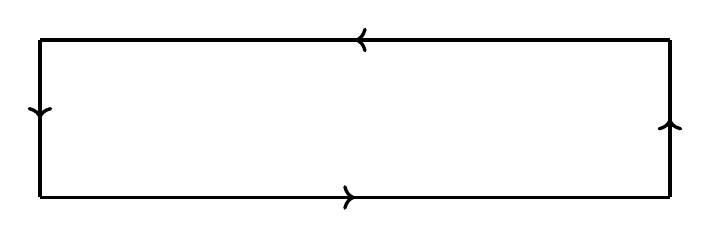
\begin{tikzpicture}
\begin{scope}[very thick,decoration={
    markings,
    mark=at position 0.5 with {\arrow{>}}}
    ] 
    \draw[postaction={decorate}] (-4,0)--(4,0);
    \draw[postaction={decorate}] (4,0)--(4,2);
    \draw[postaction={decorate}] (4,2)--(-4,2);
    \draw[postaction={decorate}] (-4,2)--(-4,0);
\end{scope}
\end{tikzpicture}

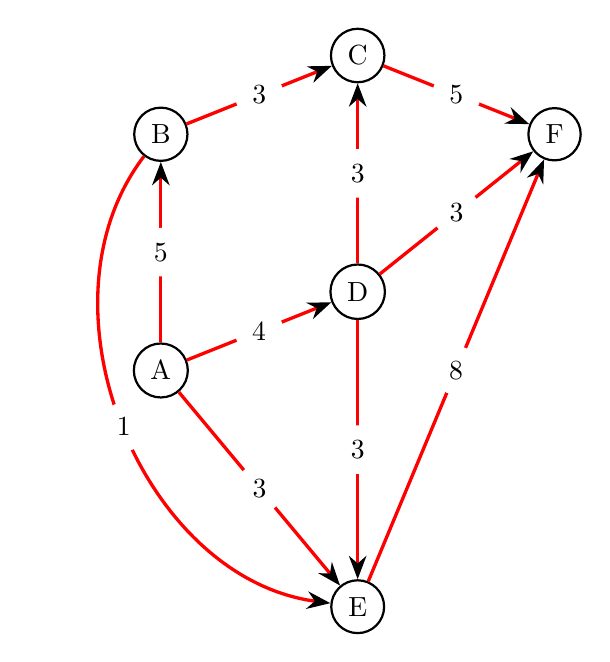
\begin{tikzpicture}
\begin{scope}[every node/.style={circle,thick,draw}]
    \node (A) at (0,0) {A};
    \node (B) at (0,3) {B};
    \node (C) at (2.5,4) {C};
    \node (D) at (2.5,1) {D};
    \node (E) at (2.5,-3) {E};
    \node (F) at (5,3) {F} ;
\end{scope}

\begin{scope}[>={Stealth[black]},
              every node/.style={fill=white,circle},
              every edge/.style={draw=red,very thick}]
    \path [->] (A) edge node {$5$} (B);
    \path [->] (B) edge node {$3$} (C);
    \path [->] (A) edge node {$4$} (D);
    \path [->] (D) edge node {$3$} (C);
    \path [->] (A) edge node {$3$} (E);
    \path [->] (D) edge node {$3$} (E);
    \path [->] (D) edge node {$3$} (F);
    \path [->] (C) edge node {$5$} (F);
    \path [->] (E) edge node {$8$} (F); 
    \path [->] (B) edge[bend right=60] node {$1$} (E); 
\end{scope}
\end{tikzpicture}


%	\begin{figure}[h]
%	\centering
%	\includegraphics[width=0.35\textwidth]{graph1.jpg}
%	\end{figure}

\begin{enumerate}[(a)]
\item Is the graph $G$ connected? Explain.
\item Is $d7e4b1a2c5f8g$ a trail? Explain. Is it a path? Explain.
\item Is $c5f8g6c2a$ a path? Explain. Is this walk closed? Explain.
\item Does this graph have a circuit? Explain. 
\item Let $A_G$ denote the adjacency matrix of $G$. Given the following:
	\[
	A_G^{10}=
	\begin{pmatrix}
	860 & 746 & 746 & 681 & 681 & 681 & 681 \\
	746 & 1282 & 940 & 884 & 884 & 543 & 543 \\
	746 & 940 & 1282 & 543 & 543 & 884 & 884 \\
	681 & 884 & 543 & 743 & 742 & 401 & 401 \\
	681 & 884 & 543 & 742 & 743 & 401 & 401 \\
	681 & 543 & 884 & 401 & 401 & 743 & 742 \\
	681 & 543 & 884 & 401 & 401 & 742 & 743
	\end{pmatrix}
	\]
How many closed walks of length 10 are there starting at $a$? Explain. 
\end{enumerate} \pspace

\sol 
\begin{enumerate}[(a)]
\item The graph $G$ is connected because between any distinct vertices $v, w$, there is a walk from $v$ to $w$. \pspace

\item This walk does not repeat an edge. Therefore, this walk is a trail. Because this walk does not repeat an edge or a vertex, this walk is also a path. \pspace

\item This walk is not a path because the vertex $c$ is repeated. This walk is also open and not closed because the walk does not start and end at the same point. \pspace

\item This graph has six circuits. For instance, the walk $b3d7e4b$ is a circuit. \pspace

\item A closed walk is a walk that starts and ends at the same point. So a closed walk starting at $a$ must also end at $a$. Therefore, we need find the number of walks of length 10 from $a$ to itself. We know the number of walks from $v_i$ to $v_j$ of length $k$ is the $a_{ij}$ entry of $A_G^k$. Therefore, the number of walks from $a$ to $a$ is the $a_{11}$ entry of $A_G^{!0}$. We can see there are 860 walks of length 10 from $a$ to $a$. 
\end{enumerate}



\newpage



% Problem 2
\problem{10} Consider the graph $G$ shown below.
	\begin{figure}[h]
	\centering
	\includegraphics[width=0.14\textwidth]{graph2.jpg}
	\end{figure}

\begin{enumerate}[(a)]
\item Does there exist a Hamiltonian circuit for this graph? Explain. 
\item Does there exist an Euler circuit for this graph? Explain. 
\item Find the adjacency matrix for this graph.
\item Find the number of walks from $a$ to $b$ of length 4. Be sure to justify your answer. 
\end{enumerate} \pspace

\sol 
\begin{enumerate}[(a)]
\item A Hamiltonian circuit is a simple circuit (a closed walk with at least one edge and no repeated edge nor repeated vertex---except the first and last) that includes every vertex of $G$. The walk $b3a1d8e7c5b$ includes every vertex of $G$, starts and stops at the same vertex (a closed walk), and has no repeated edge or vertex (except the first and last). Therefore, $G$ has a Hamiltonian circuit. \pspace
 
\item An Euler circuit is a circuit (a closed walk with at least one edge that does not contain a repeated edge) that includes every every edge (and hence every vertex) of $G$. If a graph $G$ has an Euler circuit, then one can begin the circuit at any vertex.\footnote{If the Euler circuit is $v_0 e_0 v_1 e_1 \cdots e_{i-1} v_i e_i v_{i+1} e_{i+1} \cdots e_{n-1}v_0$ and one wishes to begin at $v_i$, one can use the Euler circuit $v_i e_i v_{i+1} e_{i+1} \cdots e_{n-1} v_0 e_0 v_1 e_1 \cdots e_{i-1} v_i$.} Without loss of generality, assume the Euler circuit begins at $b$. One must then move alone 3 to $a$. If one then moves along 2 to $b$, then one must repeat edge 3 to walk to the remaining vertices of $G$. Therefore, if one begins at $b$, one must move along 3 to $a$. One then must move along 1 to $d$ and then along 8 to $e$. One must then either travel along edge 4 or 7. If one travels along 4, then one must either travel along vertex 2---which again forces a repetition of edge 3---or travel along edge 1, which is a repeated edge. Therefore, one must travel along 7 to vertex $c$. One can then only travel along vertex 5 or 6. If one travels along edge 5, then one must repeat edge 3. If one travels along edge 6, then one must repeat edge 8. But then one cannot proceed from vertex $c$---which is not the starting vertex---without repeating an edge. Therefore, $G$ cannot have an Euler circuit. Alternatively, recall that a directed graph has an Euler circuit if and only if the graph is connected and $\deg^+ v= \deg^- v$ for all $v \in V(G)$. Observe that that the graph $G$ is connected. However, observe that $\deg^-(b)= 2 \neq 1= \deg^+(b)$. Therefore, $G$ does not have an Euler circuit. \pspace

\item Recall that the adjacency matrix for a graph $G$, $A_G$, is the matrix given by $A_G= (a_{ij})$, where $a_{ij}$ is the number of edges from $v_i$ to $v_j$. Ordering the vertices as $a, b, c, d, e$, the adjacency matrix is\dots
	\[
	A_G= 
	\begin{pmatrix}
	0 & 1 & 0 & 1 & 0 \\
	1 & 0 & 0 & 0 & 0 \\
	0 & 1 & 0 & 1 & 0 \\
	0 & 0 & 0 & 0 & 1 \\
	1 & 0 & 1 & 0 & 0 
	\end{pmatrix}
	\]

\item The number of walks from $v_i$ to $v_j$ of length $k$ is the $a_{ij}$ entry of the matrix $A_G^k$, where $A_G$ is the adjacency matrix of $G$. We have\dots
	\[
	\begin{aligned}
	A_G&= 
	\begin{pmatrix}
	0 & 1 & 0 & 1 & 0 \\
	1 & 0 & 0 & 0 & 0 \\
	0 & 1 & 0 & 1 & 0 \\
	0 & 0 & 0 & 0 & 1 \\
	1 & 0 & 1 & 0 & 0 
	\end{pmatrix} \\[0.3cm]
	A_G^2&= 
	\begin{pmatrix}
	1 & 0 & 0 & 0 & 1 \\
	0 & 1 & 0 & 1 & 0 \\
	1 & 0 & 0 & 0 & 1 \\
	1 & 0 & 1 & 0 & 0 \\
	0 & 2 & 0 & 2 & 0 
	\end{pmatrix} \\[0.3cm]
	A_G^4= (A_G^2)^2&= 
	\begin{pmatrix}
	1 & 2 & 0 & 2 & 1 \\
	1 & 1 & 1 & 1 & 0 \\
	1 & 2 & 0 & 2 & 1 \\
	2 & 0 & 0 & 0 & 2 \\
	2 & 2 & 2 & 2 & 0 
	\end{pmatrix}
	\end{aligned}
	\]
Therefore, the number of walks from $a$ to $b$ of length 4 is the $a_{12}$ entry of $A_G^4$, which is 2. There are two walks of length four from $a$ to $b$. We can find all such walks: $a1d8e7c5b$ and $a1d8e4a2b$.
\end{enumerate}



\newpage



% Problem 3
\problem{10} Consider the graph $G$ shown below.
	\begin{figure}[h]
	\centering
	\includegraphics[width=0.3\textwidth]{graph3.jpg}
	\end{figure}

\begin{enumerate}[(a)]
\item Does there exist an Euler trail for this graph? If so, find one. If not, explain why.
\item Does there exist an Euler circuit for this graph? If so, find one. If not, explain why. 
\item Does there exist a Hamiltonian circuit for this graph? If so, find one. If not, explain why. 
\end{enumerate} \pspace

\sol 
\begin{enumerate}[(a)]
\item For an undirected graph $G$, there exists an Euler trail in $G$ if and only if $G$ is connected and there are exactly two vertices of odd degree. If $G$ has an Euler trail, it must be between the vertices with odd degree. First, observe that $G$ is connected. Finally, observe that the degree of every vertex of $G$ is even except the middle two vertices. Therefore, there exists an Euler trail for $G$. 

\item For an undirected graph $G$, there exists an Euler circuit in $G$ if and only if $G$ is connected and every vertex has positive even degree. Observe that the `middle' two vertices of $G$ have odd degree. Therefore, $G$ does not have an Euler circuit. 



\end{enumerate}



\newpage



% Problem 4
\problem{10} Showing all your work and fully justifying your reasoning, respond to the following:
	\begin{enumerate}[(a)]
	\item Does there exist a tree with 2023 vertices and 2024 edges? Explain. 
	\item Does a graph with five vertices and four edges have to be a tree? Explain.
	\item Find two non-isomorphic trees with five vertices. Be sure to explain why they cannot be isomorphic. 
	\end{enumerate}


\end{document}